% !TEX root = ../main.tex
\section{PIN codes vs. Android Unlock Patterns}

  One of the well known password mechanisms are the 4-digit PIN code. These codes are commonly used for accessing banking systems, using payment cards, and locking mobile screens for unauthorized access in the same way as android unlock patterns are used. The 4-digit PIN have been research before, but have not been compared in detail. This section will briefly go through a big dataset of PIN codes to see if there are related characteristic user behavior in the usage of both. 

  The data set used contains 204,432 4-digit PIN codes \cite{danielamitay} collected from an mobile application called "Big Brother Camera security" \cite{bigbrother} created by Daniel Amitay. The application is a screen lock mechanism using a 4-digit PIN code with the extra feature of taking a picture of the person typing the pattern if wrongly typed more then 3 times. The PIN codes used in the Big Brother application. Daniel Amitay have granted permission to use his data set for comparing android pattern locks and and 4-digit PIN in this master thesis. 

  Figure \ref{fig:top10pins} is a graph showing the freqency of the top 10 patterns. The pattern with most occurences constitues about 4.34\% of the data set.
  In total, top 10 patterns constitues 14.45\% of all patterns in the data set. By studying the codes in the top 10 list, 4 out of 10 codes do all have a digit repeated four times. The top code is 1234, that is a numerical sequence that is easy to remember. There are some codes that at first sight seems random, but realy are not. Codes like 2580 have a practical explanation to be in top 10 list because that is the only code than forms a straight line of 4 digits on the keypad. The code 5683 have a more semantic meaning than just the numbers because the code forms the word "love" on the keypad. The last code in the list is 1998 that is the probably the date of birth of the users using the application. Figure \ref{fig:pindecades} will look at the frequent use of PIN codes corresponds to specific year.

  \begin{figure}[H]
    \centering
    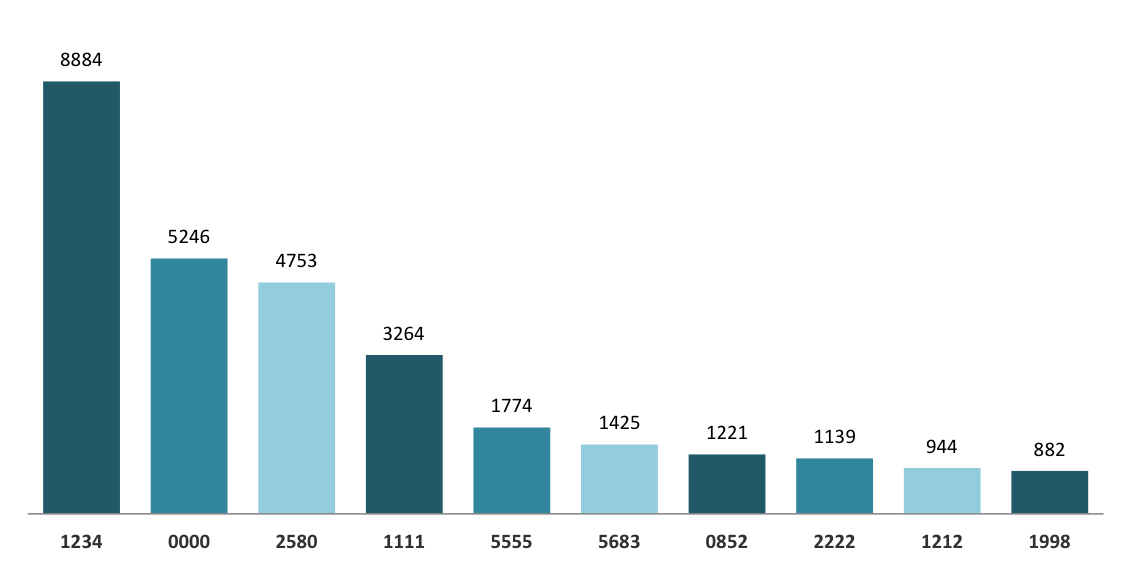
\includegraphics[width=\textwidth]{pics/analysis/top10pin.png}
    \caption{Top 10 PIN codes}
    \label{fig:top10pins}
  \end{figure}

  Figure \ref{fig:pindecades} is the distribution of PIN codes from different decades. 
    
  \begin{figure}[H]
    \centering
    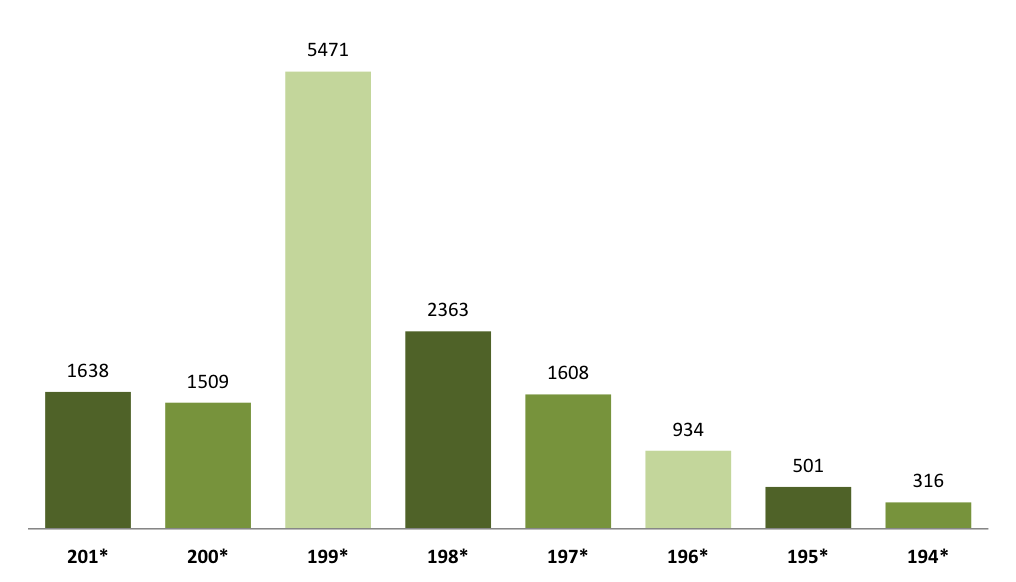
\includegraphics[width=\textwidth]{pics/analysis/pindecades.png}
    \caption{PIN codes by decade}
    \label{fig:pindecades}
  \end{figure}

  Figure \ref{fig:datagenetics} is a hetmap plot of 3,4 million PIN codes \cite{datagenetics}. The x-axis is the two first digits in the PIN code and the two last digits in the PIN code are on the y-axis, so each pixel in the plot correspond to a PIN code and the colors indicate the frequency. The yellow color indicates high frequency while the red color indicates low frequency. 

  There are 3 main observations in the heatmap that are worth noticing. The first observation is that there is a crossing yellow line starting from code 0000 and ending up in the code 9999. The codes on that line are repeating codes like 1212 and 0000. There are some spots on that line that occur with a brither color repeating for each 11 code. This are the codes that have all four digits the same, like 0000 and 5555. The corner on the bottom left have a big yellow area that actually are PIN codes forming a date with either the format DDMM or MMDD. There is also a stright vertical line with a high density with patterns starting with 19 and 20. The line is corresponding to decades starting with 19** and 20**. This is related with the plot of PIN codes corresponding to decades in Figure \ref{fig:pindecades}.

  \begin{figure}[H]
    \centering
    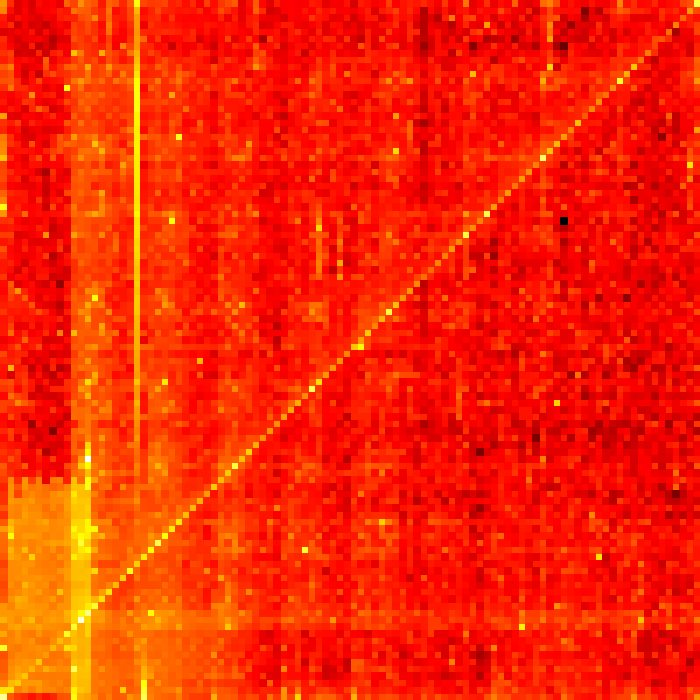
\includegraphics[width=0.6\textwidth]{pics/analysis/datagenetics.jpg}
    \caption{PIN codes plotted in heatmap \cite{datagenetics}}
    \label{fig:datagenetics}
  \end{figure}

  \begin{figure}[H]
    \centering
    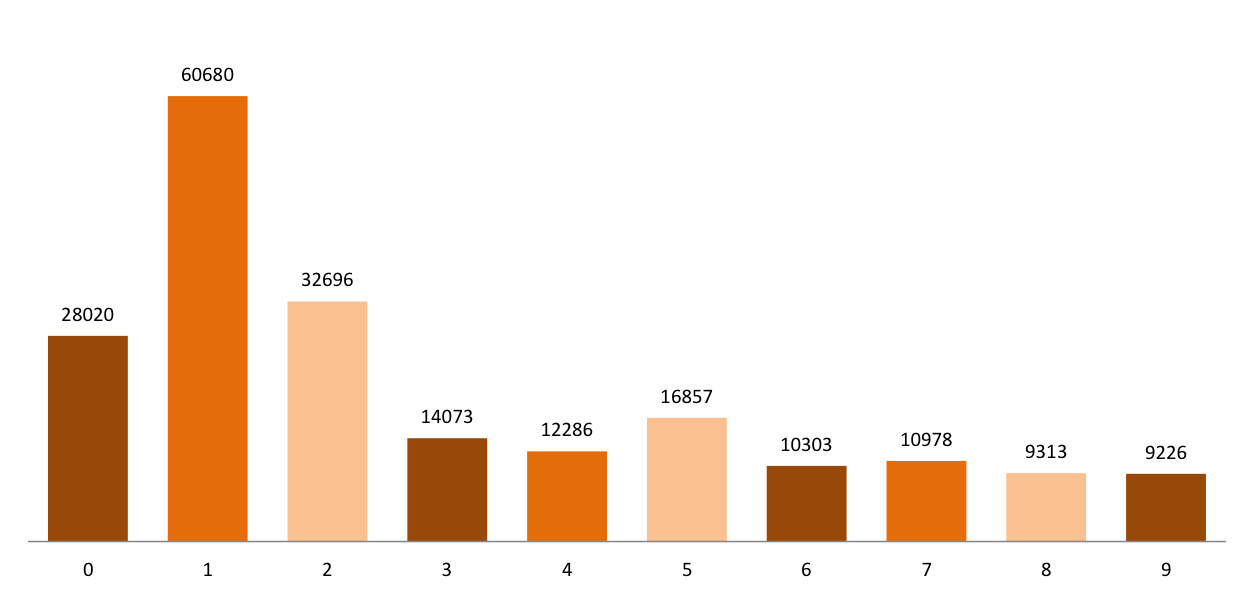
\includegraphics[width=\textwidth]{pics/analysis/pinstart.png}
    \caption{PIN code starting point}
    \label{fig:pinstart}
  \end{figure}

  \begin{figure}[H]
    \centering
    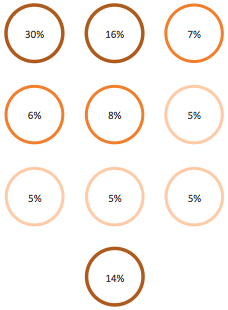
\includegraphics[width=0.40\textwidth]{pics/analysis/startpointpin.png}
    \caption{PIN code starting points}
    \label{fig:pinstart2}
  \end{figure}

